\documentclass[aspectratio=169,11pt]{beamer}
\usepackage{luatexja}
\usepackage{luatexja-fontspec}
\usepackage{amsmath,amssymb,bm}
\usepackage{booktabs}
\usepackage{tikz}
\usetikzlibrary{arrows.meta,positioning,calc,shapes.geometric}
\usetheme{Madrid}
\usecolortheme{seahorse}
\setbeamertemplate{navigation symbols}{}
\setbeamertemplate{footline}[frame number]
\definecolor{mainblue}{RGB}{22,76,125}
\definecolor{accent}{RGB}{186,93,45}
\definecolor{soft}{RGB}{242,246,250}
\setbeamercolor{title}{fg=mainblue}
\setbeamercolor{frametitle}{fg=mainblue}
\setbeamercolor{block title}{bg=mainblue!12,fg=mainblue}
\setbeamercolor{block body}{bg=soft,fg=black}
\setbeamercolor{alerted text}{fg=accent}
\setbeamerfont{title}{size=\Large,series=\bfseries}
\setbeamerfont{frametitle}{size=\large,series=\bfseries}
\setbeamerfont{block title}{series=\bfseries}
\setbeamerfont{normal text}{size=\normalsize}
\setlength{\parskip}{0.3em}
\newcommand{\key}[1]{\textcolor{accent}{\bfseries #1}}
\newcommand{\smallcite}[1]{{\scriptsize\color{gray}#1}}

\title{研究業績と再任後の研究計画}
\subtitle{量子エンタングルメント・対称性・トポロジーから見る量子多体系の創発}
\author{沼澤 宙朗}
\institute{東京大学物性研究所}
\date{}

\begin{document}

\begin{frame}
  \titlepage
\end{frame}

\begin{frame}{本日のメッセージ}
\begin{block}{中心的な問い}
\centering
\Large 複雑な量子系において、\key{量子エンタングルメント}は\key{どのような創発自由度・相転移}を生み出すのか。
\end{block}
\vspace{0.4em}
\begin{columns}[T]
\column{0.31\textwidth}
\begin{block}{基礎概念}
エンタングルメント\\対称性\\トポロジー\\ゲージ原理
\end{block}
\column{0.31\textwidth}
\begin{block}{対象}
量子多体系\\強相関系\\開放量子系\\非平衡ダイナミクス
\end{block}
\column{0.31\textwidth}
\begin{block}{目標}
普遍法則の抽出\\相・相転移の分類\\物性と量子情報の接続
\end{block}
\end{columns}
\end{frame}

\begin{frame}{研究の流れ：エンタングルメントから開放系へ}
\centering
\begin{tikzpicture}[x=1cm,y=1cm,>=Latex]
\draw[thick,mainblue] (0,0) -- (11.6,0);
\foreach \x/\t/\d in {0.5/{キャリア前半}/{エンタングルメントと創発},4.2/{基礎言語}/{CFT・量子情報・統計物理},7.9/{キャリア後半}/{量子開放系の普遍性},11.1/{今後}/{統一的分類と実験接続}}{
  \fill[accent] (\x,0) circle (2.5pt);
  \node[align=center,above=0.25cm] at (\x,0) {\bfseries \t};
  \node[align=center,below=0.35cm,text width=2.6cm] at (\x,0) {\small \d};
}
\end{tikzpicture}
\vspace{1.1em}
\begin{block}{一貫した視点}
場の量子論を基礎言語に、量子情報と統計物理を取り込み、\key{創発現象の普遍性}を体系的に理解する。
\end{block}
\end{frame}

\begin{frame}{業績 1：エンタングルメントと創発ゲージ構造}
\begin{columns}[T]
\column{0.57\textwidth}
\begin{block}{主な成果}
\begin{itemize}
  \item 格子スピン模型からゲージ理論が創発する場合の\key{エンタングルメント・エントロピーの一般公式}を導出。
  \item 創発ゲージ場に特有な古典情報量、すなわち\key{シャノン項}を同定。
  \item 分数量子ホール効果、スピン液体、トポロジカル秩序に現れる分数化励起の情報論的理解に接続。
\end{itemize}
\end{block}
\column{0.38\textwidth}
\begin{block}{物理的意義}
\centering
\begin{tikzpicture}[node distance=0.8cm,>=Latex]
\node[draw,rounded corners,fill=soft,text width=3.3cm,align=center] (spin) {格子量子多体系};
\node[draw,rounded corners,fill=soft,text width=3.3cm,align=center,below=of spin] (gauge) {創発ゲージ自由度};
\node[draw,rounded corners,fill=soft,text width=3.3cm,align=center,below=of gauge] (info) {エンタングルメント\\+ シャノン項};
\draw[->,thick,mainblue] (spin) -- (gauge);
\draw[->,thick,mainblue] (gauge) -- (info);
\end{tikzpicture}
\end{block}
\end{columns}
\smallcite{提出書類：業績 A-27、添付論文 1}
\end{frame}

\begin{frame}{業績 2：テンソルネットワークと連続幾何}
\begin{columns}[T]
\column{0.52\textwidth}
\begin{block}{cMERA による連続極限}
テンソルネットワークの連続極限を用い、エンタングルメントの階層構造から\key{連続幾何が自然に現れる}ことを示した。
\end{block}
\begin{block}{位置づけ}
量子情報幾何・変分法に基づき、強相関系の量子情報構造を幾何学的に捉える基盤を構築。
\end{block}
\column{0.43\textwidth}
\centering
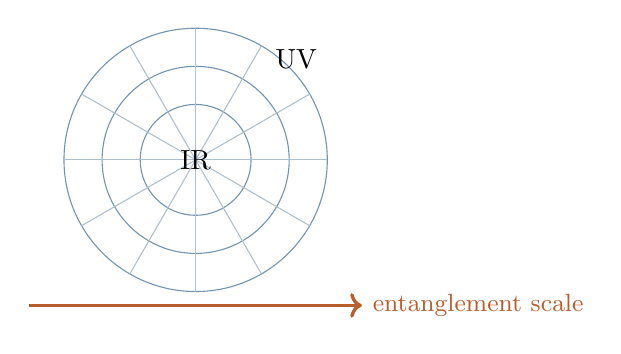
\begin{tikzpicture}[scale=0.88]
\foreach \r in {0.8,1.35,1.9}{\draw[mainblue!60] (0,0) circle (\r);}
\foreach \a in {0,30,...,330}{\draw[mainblue!35] (0,0) -- (\a:1.9);}
\node at (0,0) {IR};
\node at (1.45,1.45) {UV};
\draw[->,very thick,accent] (-2.4,-2.1) -- (2.4,-2.1) node[right]{\small entanglement scale};
\end{tikzpicture}
\vspace{0.5em}
{\small エンタングルメント階層 $\Rightarrow$ 幾何}
\end{columns}
\smallcite{提出書類：業績 A-26}
\end{frame}

\begin{frame}{業績 3：開放系エンタングルメント相転移}
\begin{columns}[T]
\column{0.56\textwidth}
\begin{block}{発見}
一次元フェルミオン系の非エルミートダイナミクスを解析し、エンタングルメントの時間発展が\key{2 次の相転移}を起こす開放系特有の臨界現象を発見。
\end{block}
\begin{block}{意義}
非エルミート効果が、エンタングルメント生成と量子情報流に与える影響を理論的に明確化。
\end{block}
\column{0.39\textwidth}
\centering
\begin{tikzpicture}[x=1.0cm,y=0.8cm]
\draw[->] (0,0) -- (4.5,0) node[right] {$g$};
\draw[->] (0,0) -- (0,3.1) node[above] {$S(t)$};
\draw[very thick,mainblue] (0.25,0.45) .. controls (1.2,0.55) and (1.7,0.75) .. (2.1,1.3) .. controls (2.4,1.95) and (3.1,2.35) .. (4.1,2.45);
\draw[dashed,accent,thick] (2.15,0) -- (2.15,2.7);
\node[accent] at (2.15,-0.35) {$g_c$};
\node[align=center] at (3.1,1.0) {開放系の\\臨界性};
\end{tikzpicture}
\end{columns}
\smallcite{提出書類：業績 A-9、PRX 掲載、引用 200 件超}
\end{frame}

\begin{frame}{業績 4：開放 SYK 模型と強相関散逸系}
\begin{block}{ラージ $N$ 極限で可解な開放強相関模型}
強相関系の代表である SYK 模型を開放系へ拡張し、非平衡経路積分により、散逸を含みながら解析可能なプラットフォームを構築。
\end{block}
\begin{columns}[T]
\column{0.48\textwidth}
\begin{block}{得られた物理}
\begin{itemize}
  \item 散逸下のカオス性とデコヒーレンスの競合
  \item 量子ダイナミクスが誘起する\key{動的相転移}
  \item 相転移を\key{離散対称性の自発的破れ}として理解
\end{itemize}
\end{block}
\column{0.47\textwidth}
\begin{block}{一般化}
時間反転対称性・離散対称性の分類、量子アノマリー、量子チャンネル固有値統計に接続し、開放系の普遍性クラス構築へ。
\end{block}
\end{columns}
\smallcite{提出書類：業績 A-11, A-7, A-5}
\end{frame}

\begin{frame}{これまでの成果の統合的な位置づけ}
\centering
\begin{tikzpicture}[>=Latex,node distance=1.35cm]
\node[draw,rounded corners,fill=soft,text width=3.2cm,align=center] (ent) {エンタングルメント};
\node[draw,rounded corners,fill=soft,text width=3.2cm,align=center,right=of ent] (sym) {対称性・アノマリー};
\node[draw,rounded corners,fill=soft,text width=3.2cm,align=center,below=of ent] (top) {トポロジー・ゲージ構造};
\node[draw,rounded corners,fill=soft,text width=3.2cm,align=center,right=of top] (open) {非平衡・開放系};
\node[draw,rounded corners,fill=accent!15,text width=4.4cm,align=center,below right=0.7cm and -1.2cm of top] (goal) {量子多体系における\\創発現象の普遍性};
\draw[->,thick,mainblue] (ent) -- (sym);
\draw[->,thick,mainblue] (ent) -- (top);
\draw[->,thick,mainblue] (sym) -- (open);
\draw[->,thick,mainblue] (top) -- (open);
\draw[->,thick,accent] (open) -- (goal);
\draw[->,thick,accent] (top) -- (goal);
\end{tikzpicture}
\vspace{0.5em}
\begin{block}{次のステップ}
この統一的視点を、物性・量子情報・統計物理を横断する\key{新しい理論体系}へ発展させる。
\end{block}
\end{frame}

\begin{frame}{再任後の研究計画：三つの柱}
\begin{columns}[T]
\column{0.31\textwidth}
\begin{block}{1. 開放量子系}
臨界現象・相の分類\\対称性に基づく秩序変数\\量子アノマリー
\end{block}
\column{0.31\textwidth}
\begin{block}{2. 開放強相関系}
開放 SYK の発展\\ハバード模型等への応用\\界面・不純物問題
\end{block}
\column{0.31\textwidth}
\begin{block}{3. トポロジカル相}
創発ゲージ構造\\量子誤り訂正\\分数化励起・アノマリー
\end{block}
\end{columns}
\vspace{0.7em}
\begin{block}{全体目標}
\centering
エンタングルメント・非平衡・強相関・トポロジーを軸に、\key{量子技術時代の普遍的原理}を明らかにする。
\end{block}
\end{frame}

\begin{frame}{計画 1：開放量子系における普遍性と相の分類}
\begin{block}{背景}
量子計測、粒子ロス、ゲイン、環境結合は現代の量子技術で不可避であり、従来の平衡統計力学・バンド理論を超えた枠組みが必要。
\end{block}
\begin{block}{具体的課題}
\begin{itemize}
  \item 開放系における臨界現象の分類
  \item 非平衡開放系のランダウ・ギンツブルグ理論の構築
  \item 対称性の自発的破れ・量子アノマリーの分類
  \item 場の量子論を用いた開放系相構造の解明
\end{itemize}
\end{block}
\begin{alertblock}{実験との接続}
量子光学・フォトニクスにおける PT 対称性、例外点などの非エルミート現象と連携。
\end{alertblock}
\end{frame}

\begin{frame}{計画 2：強相関系における量子開放ダイナミクス}
\begin{columns}[T]
\column{0.54\textwidth}
\begin{block}{研究の方向}
\begin{itemize}
  \item 開放強相関系の新しい相を探索
  \item 平均場近似・グリーン関数法を開放系へ拡張
  \item ハバード模型など現実的模型への応用
  \item 不純物・界面の非平衡理論を構築
  \item 非フェルミ流体の有効場理論を非平衡へ展開
\end{itemize}
\end{block}
\column{0.41\textwidth}
\begin{block}{期待される波及}
量子ドット、超伝導接合、光学系など、散逸と相互作用が同時に効く実験系に対して、強相関物性の新しい設計原理を与える。
\end{block}
\end{columns}
\end{frame}

\begin{frame}{計画 3：トポロジカル相と量子情報}
\begin{block}{基本思想}
エンタングルメントは多体系の自由度を再構成し、有効ゲージ自由度・トポロジカル秩序・分数化励起を生み出す。
\end{block}
\begin{columns}[T]
\column{0.47\textwidth}
\begin{block}{理論的課題}
\begin{itemize}
  \item 創発トポロジカル秩序の一般理論
  \item 分数化励起・アノマリーと量子情報の関係
  \item ゲージ理論の非平衡ダイナミクス
\end{itemize}
\end{block}
\column{0.47\textwidth}
\begin{block}{応用・連携}
\begin{itemize}
  \item 量子誤り訂正符号
  \item 量子ホール効果・スピン液体
  \item フォトニクス・物質中の光学応答
\end{itemize}
\end{block}
\end{columns}
\end{frame}

\begin{frame}{物性研究所で展開する意義}
\begin{block}{理論と実験の接点}
物性研究所の実験基盤と連携し、非エルミート現象、強相関散逸系、トポロジカル物性を理論・実験の両面から統合的に理解する。
\end{block}
\begin{columns}[T]
\column{0.31\textwidth}
\begin{block}{物性物理}
強相関・非平衡・トポロジカル相
\end{block}
\column{0.31\textwidth}
\begin{block}{量子情報}
エンタングルメント・誤り訂正・量子計測
\end{block}
\column{0.31\textwidth}
\begin{block}{統計物理}
普遍性・相転移・有効場理論
\end{block}
\end{columns}
\vspace{0.6em}
\begin{alertblock}{貢献}
分野横断的な理論基盤を構築し、量子デバイス時代の物性理論を推進する。
\end{alertblock}
\end{frame}

\begin{frame}{教育・研究指導の方針}
\begin{block}{学生の成長プロセス}
\centering
\begin{tikzpicture}[>=Latex,node distance=1.0cm]
\node[draw,rounded corners,fill=soft,text width=2.8cm,align=center] (a) {初期：明確なテーマ設定};
\node[draw,rounded corners,fill=soft,text width=2.8cm,align=center,right=of a] (b) {中期：基礎技術と文献読解};
\node[draw,rounded corners,fill=soft,text width=2.8cm,align=center,right=of b] (c) {後期：独立したテーマ発見};
\node[draw,rounded corners,fill=soft,text width=2.8cm,align=center,right=of c] (d) {発信：論文・国際交流};
\draw[->,thick,mainblue] (a) -- (b);
\draw[->,thick,mainblue] (b) -- (c);
\draw[->,thick,mainblue] (c) -- (d);
\end{tikzpicture}
\end{block}
\begin{block}{方針}
自身の海外経験を活かし、学生・研究員が国際的な研究環境を経験し、独立した研究者へ成長できるよう支援する。
\end{block}
\end{frame}

\begin{frame}{今後のロードマップ}
\begin{columns}[T]
\column{0.31\textwidth}
\begin{block}{短期}
開放系臨界現象と対称性分類を整理し、場の理論として定式化。
\end{block}
\column{0.31\textwidth}
\begin{block}{中期}
開放強相関模型を現実的模型・界面・不純物系へ展開。
\end{block}
\column{0.31\textwidth}
\begin{block}{長期}
エンタングルメントを基軸に、非平衡・強相関・トポロジーを統合する理論体系を構築。
\end{block}
\end{columns}
\vspace{0.8em}
\begin{block}{到達目標}
\centering
物性物理と量子情報科学を結ぶ、\key{普遍性・分類・制御}の理論基盤を確立する。
\end{block}
\end{frame}

\begin{frame}{まとめ}
\begin{block}{これまで}
エンタングルメント・対称性・トポロジー・非平衡を共通言語として、創発ゲージ構造、連続幾何、開放系相転移、開放 SYK 模型を研究してきた。
\end{block}
\begin{block}{これから}
開放量子系、開放強相関系、トポロジカル相と量子情報を三本柱として、量子多体系の新しい普遍性を分類・制御する。
\end{block}
\begin{alertblock}{面接で強調する一文}
\centering
\Large 量子エンタングルメントを軸に、\key{物性物理と量子情報をつなぐ理論基盤}を構築します。
\end{alertblock}
\end{frame}

\end{document}
